\documentclass{csse4400}

\usepackage{languages}

% RUBRIC
\usepackage{multirow}
\usepackage{array}
\usepackage{xltabular}
\usepackage{pdflscape}
\usepackage{enumitem}

\newcolumntype{P}[1]{>{\centering\arraybackslash}p{#1}}
% RUBRIC

\title{TicketOverflow}
\author{Brae Webb}
\date{Semester 1, 2023}

\begin{document}
\maketitle

\section*{Summary}
In this assignment, you will demonstrate your ability to \textsl{design},
\textsl{implement}, and \textsl{deploy} a web API that can process a high load,
i.e. a scalable application.
You are to deploy an API for booking concert tickets,
generating printed tickets, and generating seating plans.
Specially your application needs to support:
\begin{itemize}
    \item Purchasing of tickets via API requests.
    \item Generation of printed (downloadable) tickets.
    \item Generation of seating plans for concerts.
    \item Providing access via a specified REST API, e.g. for use by front-end interfaces.
    \item Remaining responsive to the user while generating tickets and seating plans.
\end{itemize}

Your service will be deployed to AWS and will undergo automated correctness and load-testing to ensure it meets the requirements.

\section{Introduction}
Recent controversy has brought attention to the monopoly held by certain ticketing companies.
In hopes of an eventual collapse of the current monopoly,
we aim to develop TicketOverflow,
an online concert ticket booking system.

\paragraph{Task}
For this assignment,
you are working for TicketOverflow,
a new competitor in the online ticket booking space.
TicketOverflow uses a microservices based architecture to implement their new platform.
The CEO saw on your resume that you took Software Architecture and has assigned you to design and implement the ticket service.
This service must be scalable to cope with a large influx of bookings.

\paragraph{Requirements}
As you may be aware,
ticket booking platforms have intense peaks of traffic.
At the scale that TicketOverflow hopes to operate,
it would be inappropriate to run the servers required to meet demand at all times.
Thus, our service must be elastic --- able to scale up to meet demand and able to scale down to preserve costs.

\section{Interface}
As you are operating in a microservices context,
other service providers have been given an API specification for your service.
They have been developing their services based on this specification so you must match it exactly.

The interface specification is available to all service owners online:
\url{https://csse6400.uqcloud.net/assessment/ticketoverflow}

\section{Implementation}
The following constraints apply to the implementation of your assignment solution.

\subsection{Hamilton}
The tool to generate appropriately styled ticket and seating plan images has already been developed by the company's UX team.
TicketOverflow's investors like the designs generated by this tool.
Unfortunately, the tool developer has quit and the tool can run quite slowly.
You will have to work around this bottleneck in the design and development of your parts of the system.
(You are not allowed to reimplement or modify this tool.)

Your service must utilise the \texttt{hamilton} command line tool provided for this assignment.
You may not make any modifications to this tool.
The compiled binaries are available in the tool's GitHub repository:
\url{https://github.com/CSSE6400/hamilton}

\subsection{AWS Services}
Please make note of the \link{AWS services}
{https://labs.vocareum.com/web/2460291/1564816.0/ASNLIB/public/docs/lang/en-us/README.html#services}
that you can use in the AWS Learner Labs, and the limitations that are placed on the usage of these services.
To view this page you need to be logged in to your AWS learner lab environment and have a lab open.

\subsection{External Services}
You may \textbf{not} use services or products from outside of the AWS Learner Labs environment.
For example, you may not host instances of the \texttt{hamilton} command line tool on another cloud platform
(e.g. Google Cloud).

You may \textbf{not} use services or products that run on AWS infrastructure external to your learner lab environment.
For example, you may not deploy a third-party product like MongoDB Atlas on AWS and then use it from your service.

\section{Submission}
Your solution must committed to the GitHub repository specified in Section \ref{sec:github}.
Committing to this repository will be disabled after \textbf{16:00 (AEST) on 12 May 2022} and the contents of the repository at this time will be taken as your submission.
The repository \textbf{must} contain everything required to successfully deploy your application.
You must include all of the following in the repository:
\begin{itemize}
  \item Your implementation of the service API, including the source code and a mechanism to build the service.%
  \footnote{If you use external libraries, ensure that you pin the versions to avoid external changes breaking your application.}
  \item Terraform code that can provision your service in a fresh AWS Learner Lab environment.
  \item A \texttt{deploy.sh} script that can use your Terraform code to deploy your application.
    This script can perform other tasks as required.
\end{itemize}

When deploying your application to mark,
we will follow reproducible steps, outlined below.
You may re-create the process yourself.

\begin{enumerate}
  \item Your Git repository will be checked out locally.
  \item AWS credentials will be copied into your repository in the top-level directory,
  in a file called \texttt{credentials}.
  \item The script \texttt{deploy.sh} in the top-level of the repository will be run.
  \item The \texttt{deploy.sh} script \textbf{must} create a file named \texttt{api.txt} which contains the URL at which your API is deployed, e.g. \texttt{http://my-lb.com/}
  \item We will run automated functionality and load-testing on the URL provided in the \texttt{api.txt} file.
\end{enumerate}

\textbf{Important Note: 
Ensure your service does not exceed the resource limits of AWS Learner Labs.
For example, AWS will deactivate your account if more than 15 EC2 instances are running.}

\subsection{GitHub Repository}\label{sec:github}
You will be provisioned with a private repo on GitHub for this assignment, via GitHub Classroom.
You must click on the link below and associate your GitHub username with your UQ student ID in the Classroom.

\url{https://classroom.github.com/a/ZW_8y-7G}

\noindent
Associating your GitHub username with another student's ID,
or getting someone else to associate their GitHub username with your student ID, is \link{academic misconduct}
{https://my.uq.edu.au/information-and-services/manage-my-program/student-integrity-and-conduct/academic-integrity-and-student-conduct}.

If for some reason you have accidently associated your GitHub username with the wrong student ID,
contact the course staff as soon as possible.

\subsection{Tips}

\paragraph{If something goes wrong}
Ideally, your infrastructure will be deployed successfully but this could go wrong for any number of unforeseen reasons.
If something does go wrong during deployment,
teaching staff will refer to your \texttt{README.md} file to attempt to resolve the issue where possible.
Please ensure that your \texttt{README.md} documentation is of high quality to allow yourself the best chance for recovery.

\paragraph{Terraform plan/apply hanging}
If your \texttt{terraform plan} or \texttt{terraform apply} command hangs without any output,
check your AWS credentials.
Using credentials of an expired learner lab session will cause Terraform to hang.

\paragraph{Fresh AWS learner lab}
Your AWS learner lab can be reset using the reset button in the learner lab toolbar.
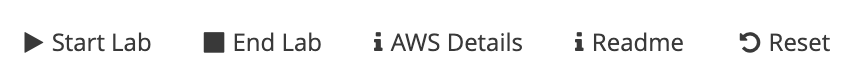
\includegraphics[width=\textwidth]{images/reset-button.png}
To ensure that you are not accidentally depending on anything specific to your learner lab environment,
we recommend that you reset your lab prior to final submission.
Note that resetting the lab can take a considerable amount of time, in the order of hours.
You should do this at least 4 to 6 hours before the submission deadline.
Please do not wait to the last minute.

\paragraph{Deploying with Docker}
In this course,
you have been shown how to use Docker containers to deploy on EC2/ECS.
You may refer to the practical worksheets for a description of how to deploy with containers \cite{prac-week5}.

%\paragraph{Unique S3 buckets}
%You may find it helpful to use S3 buckets for this assignment.
%It is important to be aware that the name of an S3 bucket has to be \textsl{globally} unique.
%To avoid any deployment conflicts,
%we recommend that you use the \texttt{random\_string} Terraform resource.
%This allows you to generate a random string which can be appended to the S3 bucket name.

%\begin{code}[language=terraform]{}
%resource "random_string" "bucket-name" {
%    length    = 16
%    special   = false
%    upper     = false
%}

%resource "aws_s3_bucket" "bucket" {
%    bucket = "my-bucket-${random_string.bucket-name.result}"
%}
%\end{code}

%\paragraph{S3 pre-signed URLs}
%If you are using AWS S3,
%ensure that you consider the security aspects of storing your files.
%You do not want to make your S3 bucket publicly accessible.
%A good middle-ground is to use \link{pre-signed URLs}{https://docs.aws.amazon.com/AmazonS3/latest/userguide/ShareObjectPreSignedURL.html} which allow you to generate temporary URLs that have read access to an object in an S3 bucket, e.g.

%\begin{code}[language=python]{}
%import boto3
%url = boto3.client('s3').generate_presigned_url(
%  ClientMethod='get_object', 
%  Params={'Bucket': BUCKET_NAME, 'Key': OBJECT_KEY},
%  ExpiresIn=3600
%)
%\end{code}

\paragraph{Authenticating AWS resources from EC2}
You may find it helpful to access other AWS resources,
such as SQS from an EC2 instance.
AWS offers \link{libraries to handle this communication}%
{https://aws.amazon.com/tools/},
however you will need to authenticate to access the resources.

You can give the EC2 instance the built-in IAM instance profile,
\texttt{LabInstanceProfile} \link{using Terraform}%
{https://registry.terraform.io/providers/hashicorp/aws/latest/docs/resources/instance\#iam_instance_profile}.
This profile will provide your EC2 instance with access to all AWS resources on the account.

%\paragraph{URL Validity}
%The URL returned from the API to access the printed ticket or seating plan
%only needs to be valid for four hours after initial generation.
%You may assume the URL will not be used after that period.
%This may be helpful if you are using signed URLs.

\subsection{Fine Print}
You can reproduce our process for deploying your application using our \link{Docker image}{https://ghcr.io/CSSE6400/csse6400-cloud-testing}:
\codefile[language=docker]{Dockerfile}{deployment/Dockerfile}

Our steps for deploying your infrastructure using this container are as follows.
\texttt{\$REPO} is the name of your repository, and
\texttt{\$CREDENTIALS} is the path where we will store our AWS credentials,
\begin{code}[language=shell]{}
$ git clone git@github.com:CSSE6400/$REPO
$ cp $CREDENTIALS $REPO
$ docker run -v /var/run/docker.sock:/var/run/docker.sock -v $(pwd)/$REPO:/workspace csse6400-cloud-testing
$ cat $REPO/api.txt # this will be used for load-testing
\end{code}

\noindent
Note that the Docker socket of the host has been mounted.
This enables running \texttt{docker} in the container.
This has been tested on MacOSX and Linux but may require WSL2 on Windows.


\section{Criteria}
Your assignment submission will be assessed on its ability to support the specified use cases.
Testing is divided into functionality testing and quality testing.
Functionality testing is to ensure that your backend software and API meet the MVP requirements by satisfying the API specification without any excessive load.
Quality testing is based upon several likely use case scenarios.
The scenarios create different scaling requirements.

Partial marks are available for both types of tests,
i.e. if some functionality is implemented you can receive marks for that functionality,
or if your service can handle 80\% of the load during quality testing you will receive marks for that.

\subsection{Functionality}
40\% of the total marks for the assignment are for correctly implementing the API specification,
irrespective of whether it is able to cope with high loads.
A suite of automated API tests will assess the correctness of your implementation, via a sequence of API calls.
Some tests from this suite will be made available before the assignment due date.

\subsection{Quality Scenarios}\label{sec:scenarios}
The remaining 60\% of the marks will be derived from how well your service handles various scenarios.
These scenarios will require you to consider how your application performs under load.
Examples of possible scenarios are described below.
These are not descriptions of specific tests that will be run,
rather they are examples of the types of tests that will be run.

\paragraph{Small concert}
As TicketOverflow is starting out,
it will need to scale to the size of a small concert.
Playhouse at QPAC is one of the first venues to sign up for the service.
Their customers purchase tickets in advance over a longer period of time.

\paragraph{Pre-sale for Hamilton}
Hamilton is now showing at the Lyric Theatre at QPAC and the pre-sale tickets are released for a limited time.
The tickets are in high demand, and there are a large number of customers trying to purchase tickets at the same time.

\paragraph{General sale for Hamilton}
The general sale for Hamilton has started, and there is a surge of customers trying to purchase tickets at the same time.
This leads to a high traffic volume on the website, which puts a strain on TicketOverflow.

\paragraph{Seating plan launch}
The frontend team at TicketOverflow have developed a new ticket purchasing interface that shows users the seating plan before they purchase.
A large concert is being used to trial this new feature.
You need to ensure that the rendering of the seating plan does not interfere with the high volume of associated ticket purchases.

\paragraph{Evening shows at QPAC}
All QPAC venues are now supported in TicketOverflow.
Each evening there are multiple concerts that run concurrently.
TicketOverflow must be able to handle a steady stream of parallel purchases, ticket generation, and seating plan generation.

\paragraph{Priority tickets}
Tickets recently went on sale for a large concert in four months time.
Some of the ticket purchasers are downloading their tickets in advance.
Meanwhile an evening show for a smaller concert is starting in a few minutes.
The evening show attendees should be able to download their tickets without being impacted by the later concert.

\paragraph{Copyright infringement}
Due to a copyright notice, ``Elsa on Ice'', has to be renamed to ``Bob on Ice''.
Unfortunately, this is a last minute name change while many users are logging in to generate their tickets.
Your system must ensure that they are not shown incorrect tickets and gracefully handles re-generation of tickets.

\paragraph{Taylor Swift tour}
Taylor Swift has chosen TicketOverflow for the release of her Eras Tour.
It is estimated that there will be about 2.8 million purchases during this time.
Your service should do its best to remain responsive during the launch of the tour.


\subsection{Marking}
Functionality accounts for 40\% of the marks for the assignment.
This is split as 25\% for correct implementation of the provided API,
and 15\% for correct generation of tickets and seating plans.
The simple queries in the API are worth much less of the mark compared to the API operations that require processing of data.

%Backend processing is the synchronous and asynchronous conversion of text to speech.
%Synchronous processing is worth 12\% and asynchronous processing is worth 8\%.
All functionality marks are based solely on correct implementation of the functionality,
as assessed by the automated functionality tests.

Scaling your application to deliver the quality scenarios accounts for the other 60\% of the marks.
The scenarios described in section \ref{sec:scenarios} provide guidance as to the type of scalability issues your system is expected to handle.
They are not literal descriptions of the exact loads that will be used.
Tests related to scenarios that involve more complex behaviour will have higher weight than other tests.

The scenarios will also evaluate whether your service is being wasteful in resource usage.
The amount of resources deployed in your AWS account will be monitored to ensure that your service implements a scaling up and scaling down procedure.

Scaling will be assessed via automated tests.
A small subset of these will be released shortly before the due date.
These tests may consume a \textbf{\emph{significant}} portion of your AWS credit.
You are advised to be prudent in how many times you execute these tests.

You will be given advanced warning of when your submission will be tested.
The idea is that it will give you a window of opportunity to confirm that your system is running correctly in your account,
before we run the automated tests.
This will also give you the opportunity to resolve any production errors that occur during testing.
For this reason,
you should ensure that your service has appropriate observability so that you can identify issues and respond accordingly.

Please refer to the marking criteria at the end of this document.


\section{Academic Integrity}
As this is a higher-level course, you are expected to be familiar with the importance of academic integrity in general, and the details of UQ's rules.
If you need a reminder, review the \link{Academic Integrity Modules}
{https://web.library.uq.edu.au/library-services/it/learnuq-blackboard-help/academic-integrity-modules}.
Submissions will be checked to ensure that the work submitted is not plagiarised.

This is an individual assignment.
You may not discuss details of approaches to solve the problem with other students in the course.
All code that you submit must be your own work.
You may not directly copy code that you have found online to solve parts of the assignment.
If you find ideas from online sources (e.g. Stack Overflow), you must \link{cite and reference}{https://web.library.uq.edu.au/node/4221/2} these sources.
Use the \link{IEEE referencing style}{https://libraryguides.vu.edu.au/ieeereferencing/gettingstarted} for citations and references.
Citations should be included in a comment at the location where the idea is used in your code.
All references for citations must be included in a file called \texttt{refs.txt}.
This file should be in the root directory of your project.

Uncited or unreferenced material will be treated as not being your own work.
Significant amounts of cited material from other sources will be considered to be of no academic merit.


\bibliographystyle{ieeetr}
\bibliography{ours}

\clearpage

\newgeometry{left=12mm,right=7mm,top=5mm,bottom=12mm}

\begin{landscape}

\fontsize{9}{11}\selectfont

\begin{xltabular}{\linewidth}{| P{1.55cm} | X | X | X | X | X | X | X |}
\hline
\multicolumn{1}{|c}{\multirow{2}{*}{\textbf{Criteria}}} &
  \multicolumn{7}{c|}{\textbf{Standard}} \\ \cline{2-8} 
\multicolumn{1}{|c}{} &
  \multicolumn{1}{c|}{\textbf{Exceptional ~ (7)}} &
  \multicolumn{1}{c|}{\textbf{Advanced ~ (6)}} &
  \multicolumn{1}{c|}{\textbf{Proficient ~ (5)}} &
  \multicolumn{1}{c|}{\textbf{Functional ~ (4)}} &
  \multicolumn{1}{c|}{\textbf{Developing ~ (3)}} &
  \multicolumn{1}{c|}{\textbf{Little Evidence ~ (2)}} &
  \multicolumn{1}{c|}{\textbf{No Evidence ~ (1)}} \\ \hline
\endhead
%
\textbf{System\newline Scope\newline20\%} &
MVP's originally proposed functional \& non-functional requirements, or those agreed \& documented early in the project, are fully delivered. &
MVP's originally proposed functional \& non-functional~require\-ments, or those agreed \& documented early in the project, are delivered with small variances. &
MVP's functional \& non-functional requirements were revised \& documented later in the project, and are almost fully delivered. &
All important functional \& non-functional requirements are delivered but some other requirements are not, whether or not original plan was revised. &
Most important functional \& non-functional requirements are delivered, whether or not original plan was revised. &
Some important functional \& non-functional requirements are delivered, whether or not original plan was revised. &
Few important functional \& non-functional requirements are delivered, whether or not original plan was revised. \\
\hline

\textbf{Architecture\newline Suitability\newline 15\%} &
Delivered architecture, supplemented by the design reflection, is very well suited to delivering all specified functional \& non-functional require\-ments, including an appropriate level of security. &
Delivered architecture, supplemented by the design reflection, is~well suited to delivering~al\-most all specified functional \& non-functional requirements, including an appropriate level of security. &
Delivered architecture, supplemented by the design reflection, is fairly well suited to delivering the key functional \& non-functional requirements, including a mostly appropriate level of security. &
Delivered architecture, supplemented by the design reflection, is capable of delivering most key functional \& non-functional requirements, including a mostly appropriate level of security. &
Delivered architecture, supplemented by the design reflection, requires workarounds in a few cases to deliver key functional \& non-functional requirements. Design has one or two obvious security issues. &
Delivered architecture, supplemented by the design reflection, requires workarounds in several cases to deliver key functional \& non-functional requirements. Design has a few obvious security issues. &
Delivered architecture, supplemented by the design reflection, makes it difficult to deliver many functional \& non-functional requirements. Design does not appear to consider security issues. \\
\hline

\textbf{Testing\newline Quality\newline 20\%} &
All functional \& non-functional requirements, \& architectural components are well tested (or are described well in a test plan) and, where feasible, are automated. &
Most key functional \& non-functional require\-ments, \& key architec\-tural components are well tested (or are described adequately in a test plan) and, where feasible, are mostly automated. &
Most key functional \& non-functional require\-ments, \& key architec\-tural components are fairly well tested (or are described fairly adequately in a test plan) and, where feasible, many are automated. &
Most key functional \& non-functional require\-ments, \& key architectural components are fairly well tested (or are described fairly adequately in a test plan) and, with some attempt at automation. &
Main test cases for most key functional \& non-functional requirements, \& key architectural components are fairly well tested (or have some informative description in a test plan). &
Main test cases for a few key functional \& non-functional requirements, \& key architectural components are moderately well tested (or have a general description in a test plan). &
Testing is poor, superficial or extremely limited. Or, extent of testing cannot be determined from submitted artefacts. \\
\hline

\textbf{Architecture\newline Description\newline 25\%} &
Clear, accurate, concise \& complete description of all aspects of the architecture. Diagrams \& narrative text complement each other. Views enhance understanding all aspects of the architecture. Choice of architecture, \& decisions about design trade-offs, are well described. &
Clear, accurate \& mostly complete description of the architecture. Diagrams \& narrative text complement each other. Views support description of the architecture. Choice of architecture, \& decisions about important design trade-offs, are well described. &
Mostly clear, accurate \& complete description of the architecture. Diagrams \& narrative text support each other. Views support some description of the architecture. Choice of architecture, \& decisions about most important design trade-offs, are adequately described. &
Fairly clear, \& mostly accurate \& complete,~des- cription of the architecture. Diagrams \&~narra- tive text are consistent. Views provide little~sup- port describing the architecture.  Choice of~archi- tecture \& decisions about some important design trade-offs, are fairly adequately described. &
Some parts of the description are unclear, in- accurate or incomplete. Most diagrams are relevant to the narrative text or a necessary diagram is missing. Justification of choice of architecture is unclear. Decisions about a few important design trade-offs are fairly adequately described. &
Some parts of the description are inaccurate or incomplete, or many parts are unclear. Some diagrams are relevant to the narrative text or a few necessary diagrams are missing. Poor justification of choice of architecture. Few design trade-offs are adequately described. &
Many parts of the description are unclear, inaccurate or incomplete. Few diagrams are relevant to the narrative text or many necessary diagrams are missing. No, or very poor, justification of choice of architecture. Trade-offs are poorly described. \\
\hline

\textbf{Architecture\newline Evaluation\newline 20\%} &
Critique \& evaluation clearly demonstrate that the delivered architecture, varied a little by the reflection comments, can deliver all functional \& non-functional requirements of the full system. &
Critique \& evaluation clearly demonstrate~that the delivered architecture, varied by the reflection comments, can deliver all functional \& non-functional requirements of the full system. &
Critique \& evaluation demonstrate that the delivered architecture, varied by the reflection comments, can deliver all important functional \& non-functional requirements of the full system. &
Critique \& evaluation demonstrate that the delivered architecture, varied by the reflection comments, can deliver all important functional \& non-functional requirements of the MVP \& part of the full system. &
Critique \& evaluation demonstrate that the delivered architecture, varied by the reflection comments, can deliver all important functional \& non-functional requirements of the MVP but little of the full system. &
Critique \& evaluation demonstrate that the delivered architecture, varied by the reflection comments, can deliver some important functional \& non-functional requirements of the MVP. &
Critique \& evaluation demonstrate that the delivered architecture, varied by the reflection comments, is unlikely to deliver most functional or non-functional requirements of the MVP. Or, they are too unclear to determine. \\
\hline

\end{xltabular}

\end{landscape}

\restoregeometry

\end{document}


